% !Mode:: "TeX:UTF-8"
\chapter{分支预测针对解耦前端的设计}

本章首先介绍前端解耦的含义,以及为什么需要对前端解耦,之后详细介绍解耦前端的设计中分支预测相关部分的设计,主要是介绍FTQ (Fetch Target Queue) 的功能和设计,FTQ作为连接分支预测部件和取指部件的关键部件,在承担保存取指请求功能的同时也承担了保存分支预测信息和管理后端指令提交信息的功能,通过FTQ能够让以Fetch Block为基本单位的分支预测部件和以单条分支为基本单位的后端流水线进行信息的交互,以实现必要的功能。

\section{香山第一版耦合前端简介}

% 还没有介绍BPU的三级覆盖预测和分支历史管理机制
% 还没有介绍IUM
% 也没有讲各个部件SRAM尺寸的改变

在香山第一版的设计中,而我们把分支预测和取指统称为流水线的前端。相对的以译码为边界,译码和译码之后的流水级我们统称为后端。而在第一版的前端设计里,取指单元和分支预测的流水级是耦合在一起的,如图\ref{fig:figure41}所示。也就是说只有当分支预测和取指单元当前流水级都完成之后,才能够流向下一流水级,这会导致分支预测和指令缓存的访问互相阻塞。例如当访问指令缓存发现miss时,即使分支预测已经完成,也仍然需要停下来等待指令缓存从下级缓存中得到回填的数据;同样的当分支预测需要覆盖预测,冲刷流水线时,即使指令缓存已经准备好被访问了,由于流水线被冲刷,暂时没有新的访问请求,也只能够等待分支预测执行。这种相互掣肘的耦合关系通过解耦,可以将大量的前端气泡消除,即将分支预测流水线和取指流水线分离,中间由一个队列连接,这个队列就是FTQ (Fetch Target Queue)。

\begin{figure}[htb]
	\centering
	\setlength\tabcolsep{3pt}  % 同一行中的图片间隔
	\vspace{5pt} % 图片上部的空白,如果太小的话,图片顶部会与正文内容十分接近
	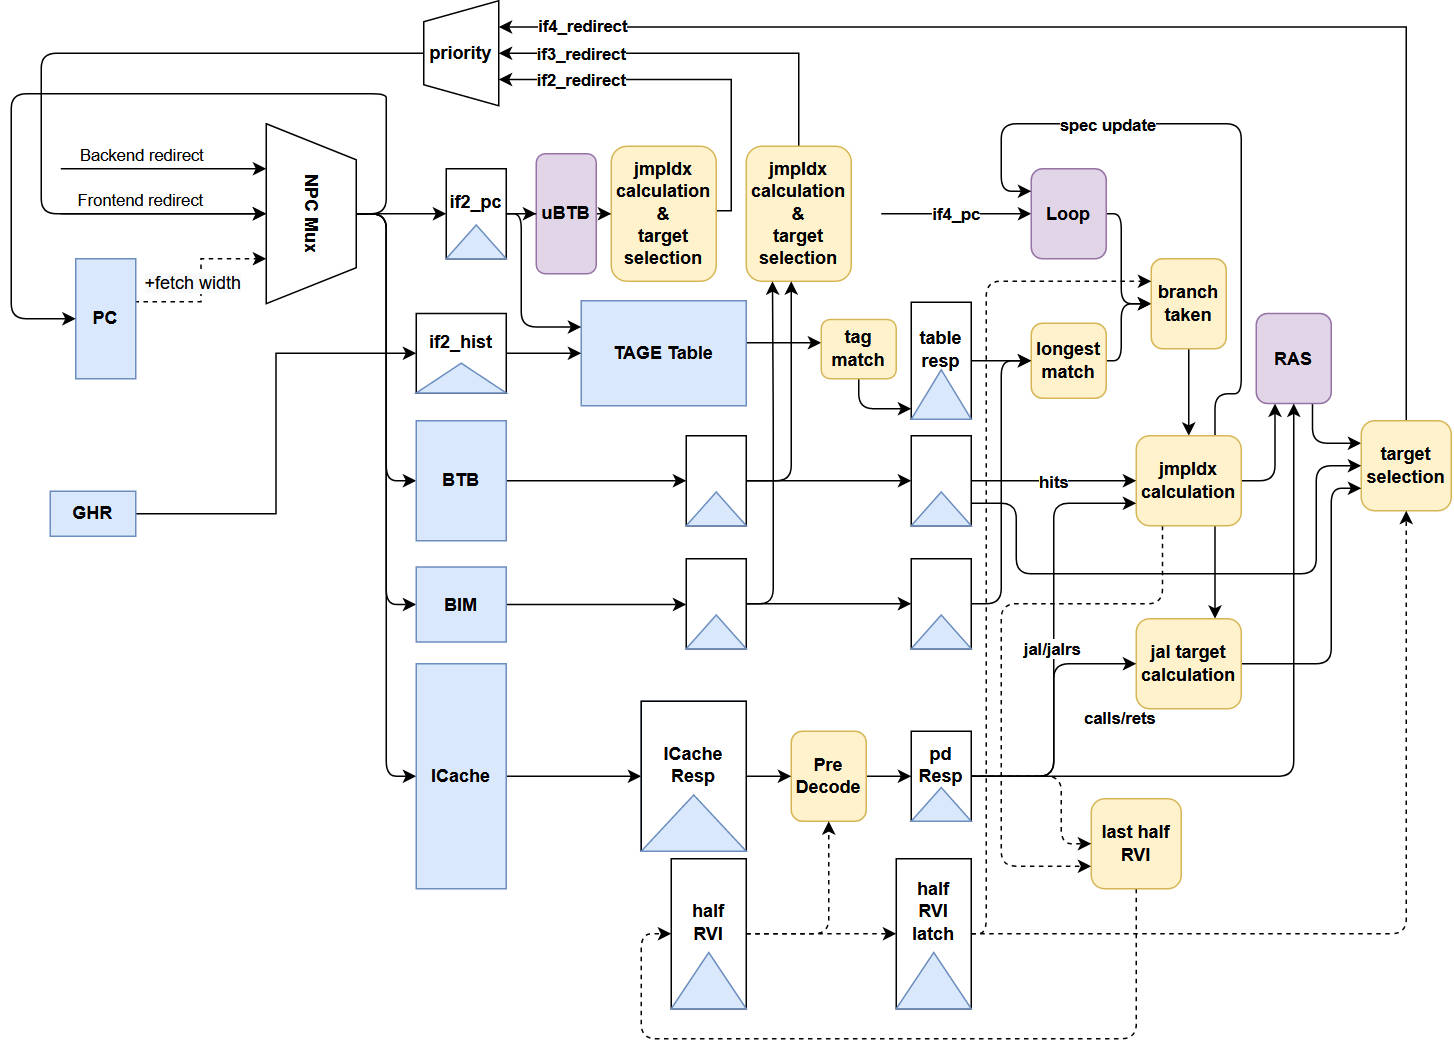
\includegraphics[width=1\textwidth]{yqh-IFU-BPU.jpg}
	\caption{香山处理器第一版分支预测与取指架构图}
    \label{fig:figure41}
\end{figure}

\section{通过FTQ实现前端解耦}

通过将分支预测流水线和取指流水线解耦开,通过FTQ连接,如图\ref{fig:figure21}所示,就能够将分支预测和取指单元变成类似于生产者和消费者的关系:分支预测作为生产者,负责不断地预测当前pc下一拍的取指pc,而不用管指令缓存是否miss,只需要将相关的取指请求放入FTQ之中。而取指单元作为消费者,负责不断地从FTQ中顺序取出取指的请求,访问指令缓存得到指令码,将它传给后端。由于在指令缓存miss时,分支预测仍旧会不断地往FTQ中送入取指请求,因此当分支预测冲刷流水线时,取指单元也不用等待,可以继续取出FTQ中之前存储的取指请求,继续访问指令缓存取指。这样一来就能够减少前端很多不必要的气泡,前端的供指效率能够得到提高,这也会对整体架构的性能有一定的正面影响

介绍FTQ的具体设计实现

\section{本章小结}

